%!TEX root = ../zeeman.tex
\subsubsection{Наблюдение нормального эффекта Зеемана}

Мы пронаблюдали характер поляризации компонент в поперечном эффекте, исследуя линию с  длиной волны  585.25 нм. Продольный эффект не изучался, так как на данной установке он не виден.

\begin{figure}[H]
	\centering
	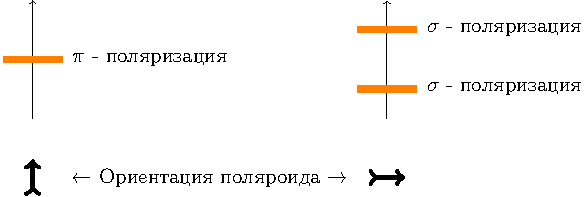
\includegraphics[scale=1]{ris/2a}
	\caption{Характер поляризации компонент}
	\label{fig:ris2a}
\end{figure}

Задав значение магнитного поля в 5520 эрстед, мы замерили расщепление линий:

\begin{figure}[H]
	\centering
	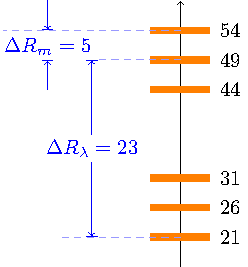
\includegraphics[scale=1]{ris/2b}
	\caption{Вид двух соседних колец интерферометра Фабри-Перо при расщеплении спектральной линии в магнитном поле в выходной плоскости спектрографа}
	\label{fig:ris2b}
\end{figure}

По формуле (\ref{eq:35}) рассчитаем $\delta\lambda$:

\begin{equation}
 	\delta \lambda=\frac{\lambda^2}{2h}\cdot\frac{5}{23}
 \end{equation} 

Здесь h=4 мм,  $\lambda$=585.25 нм:

\begin{equation}
 	\delta \lambda=\frac{342517.5625\cdot10^{-18}}{2\cdot4\cdot10^{-4}}\cdot\frac{5}{23}=9.30\cdot10^{-11} \text{ м}
 \end{equation} 

Тогда отсюда

\begin{equation}
	\Omega=\frac{2\pi c}{\lambda+\delta \lambda}-\frac{2\pi c}{\lambda-\delta \lambda}=1.024\cdot10^{11} \text{ рад/c}
\end{equation}

И в рамках классической модели (см. \ref{eq:22})

\begin{equation}
	\frac{e}{m}=\frac{2\Omega c}{H}=1.11\cdot10^{21} \text{ Кл/кг}
\end{equation}

\subsubsection{Изучение аномального эффекта Зеемана}

Аномальный эффект исследовался в <<квазинормальном>> случае, когда в спектре представлены только три компоненты --- исследуя линию с  длиной волны  607.4 нм.

Магнитное поле H=5500 эрстед.

\begin{figure}[H]
	\centering
	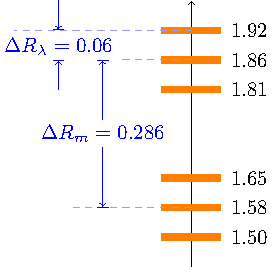
\includegraphics[scale=1]{ris/3b}
	\caption{Вид двух соседних колец интерферометра Фабри-Перо при расщеплении спектральной линии в магнитном поле в выходной плоскости спектрографа}
	\label{fig:ris3b}
\end{figure}

Теоретически посчитанное в рамках LS-приближения (\ref{eq:21})значения  g-факторов здесь
\begin{equation}
	g_1=g_2\equiv g=1+\frac12=1.5
\end{equation}

Здесь h=4 мм,  $\lambda$=607.4 нм:

\begin{equation}
 	\delta \lambda=\frac{607.4^2\cdot10^{-18}}{2\cdot4\cdot10^{-4}}\cdot\frac{0.06}{0.286}=9.67\cdot10^{-11} \text{ м}
 \end{equation} 

Тогда отсюда

\begin{equation}
	\Omega=\frac{2\pi c}{\lambda+\delta \lambda}-\frac{2\pi c}{\lambda-\delta \lambda}=1.024\cdot10^{11} \text{ рад/c}
\end{equation}